\documentclass[conference]{IEEEtran}
\IEEEoverridecommandlockouts
% The preceding line is only needed to identify funding in the first footnote. If that is unneeded, please comment it out.
\usepackage{cite}
\usepackage{amsmath,amssymb,amsfonts}
\usepackage{algorithmic}
\usepackage[]{algorithm2e}
\usepackage{caption}
\usepackage{subcaption}
\usepackage{graphicx}
\usepackage{textcomp}
\usepackage{xcolor}
\def\BibTeX{{\rm B\kern-.05em{\sc i\kern-.025em b}\kern-.08em
    T\kern-.1667em\lower.7ex\hbox{E}\kern-.125emX}}
\begin{document}

\title{Generating Synthetic Medical Images By Using WGAN To Improve CNN  Performance In Skin Cancer Classification}

\author{\IEEEauthorblockN{1\textsuperscript{st} Pooyan Sedigh }
\IEEEauthorblockA{\textit{Department of Biomedical Engineering,} \\
\textit{Science and Research Branch, Islamic Azad University,)}\\
Tehran, Iran.\\
sedigh.pooyan@taarlab.com}
\and
\IEEEauthorblockN{Rasoul Sadeghian }
\IEEEauthorblockA{\textit{Human and Robot Interaction Laboratory,} \\
Tehran, Iran. \\
rasoulsadeghian1987@gmail.com}
\and

\IEEEauthorblockN{Mehdi Tale Masouleh}
\IEEEauthorblockA{\textit{Human and Robot Interaction Laboratory, School of Electrical} \\
\textit{and Computer Engineering, University of Tehran,}\\
Tehran, Iran. \\
m.t.masouleh@ut.ac.ir}
}

\maketitle

\begin{abstract}
One of the big concern in skin cancer, is to detect the cancer with the high accuracy and so fast. In recent decade deep learning methods have led to a great breakthrough in wide range of cancer detection. 
In this paper, the Wasserstein Generative Adversarial Network(WGAN) represents to generate synthetic medical images of skin cancer. The artificial database which is obtained based on the WGAN is added to the main database and it is used for improving the performance of Convolutional Neural Network which is designed for classification of the skin cancer based on the medical images. The database which is used for this paper has just 80 images from
the International Skin Imaging Collaboration (ISIC). According to the results of implementing the designed CNN model on the test database which has 200 members, 87\% of the skin cancer images are detected correctly. \\
\end{abstract}

\begin{IEEEkeywords}
Skin cancer detection, Convlutional Neural Networks, Wasserstein Generative adversarial network, Artificial Intelligence, Neural Network
\end{IEEEkeywords}

\section{Introduction}

Cancer can be regarded as one of the main reasons of human mortality. The fast and high accurate diagnoses about cancers can reduce the risk of death among the patients~\cite{3}. According to the proposed demand, using the artificial intelligence method based on computer aid can consider as a perfect way~\cite{4}. 
In recent two decades, the significant progress in machine learning(ML) and Deep Learning (DL) algorithms and the computers' processing power have been caused a significant grows in using the proposed algorithms in different fields like medical engineering~\cite{5,6,7}. One of the main applications of ML and DL algorithms in field of medical engineering is cancer detection~\cite{8,9,10}.  According to the structure of ML and DL algorithms, having a huge database is necessary to achieve good results. Using data augmentation can solve the lack of database for medical images. Usually the data augmentation methods just consists of scale, rotation, transformation or flip, but for complex modification like pixel transformation, the GAN or WGAN algorithms are more common.
Some of algorithms which have been used for the cancer detection and classification can be regarded as, logistic regression, decision tree and Support Vector Machine (SVM)~\cite{13}. Moreover, the CNN~\cite{14,15,16}, Deep Belief Network-Neural Network (DBN-NN)~\cite{17} and Stacked Denoising Autoencoder(SDAE)~\cite{18} are widely used for detection\/ diagnosis or classification of various kinds of cancers.  By using the machine learning algorithms cancer diagnose, the cancer detection speed and quality have been increased and consequently the cancer detection's expenses may reduce, significantly.\\
The main contributions of this paper consist in, producing artificial skin cancer medical images to improve the CNN network by using WGAN. Moreover, design a CNN algorithm to use for benign and malignant skin cancer classification. Finally, assess the performance of the the designed CNN in classification of the benign and malignant skin cancer.\\
The rest of this paper is organized as follows. In Section 2,the characteristics of the data which are used for the designed WGAN for this paper are described. Then, in section 3, the process of designing GAN and WGAN algorithms and the difference of them are explained. In Section 4, the structure of CNN algorithm which is designed to use for classification of the skin cancer based on the medical images is represented. In Section 5, a deep discussion about the results of implementing the CNN algorithm on the test database is completely explained. Finally, the paper concludes with some hints and remaining as ongoing works.

\subsection{Dataset}
The preliminary database which is used for this project has just 80 members. The members of this dataset are the skin cancer images which are collected from the International Skin Imaging Collaboration (ISIC) and they are labelled as skin cancer. 
\subsection{Generating Synthetic Skin Cancer Medical Images}
In the first trace, the Generative adversarial network (GAN) algorithm is implemented on the preliminary databased in order to create the new data, to increase the number of database's members to increasing the accuracy of CNN model.The International Skin Imaging Collaboration database has some limitation for its users to download the data from it.


\begin{equation}
\nabla_{\theta_{d}}\frac{1}{m}\sum_{n=1}^{m}[\log D(x^{i})+\log(1-D(G(z^{i})))]
\label{dgan}
\end{equation}

\begin{equation}
\nabla_{\theta_{g}}\frac{1}{m}\sum_{n=1}^{m} -\log(D(G(z^{i})))
\label{ggan}
\end{equation}



\begin{equation}
\nabla_{\omega}\frac{1}{m}\sum_{n=1}^{m}[f(x^{i})-f(G(z^{i}))]
\label{cwgan}
\end{equation}




\begin{equation}
\nabla_{\omega}\frac{1}{m}\sum_{n=1}^{m} -f(G(z^{i}))
\label{gwgan}
\end{equation}

Equations~\ref{dgan} and \ref{ggan} represent the discriminator and generator functions, respectively, which are used for the GAN algorithm. 

\begin{algorithm}[t]
 \For{Under training data (s)}
 {
 \For{i$=$1 to n}{
 Input a batch of $k$ samples from random input, \{ $z^{1}, . . . ,    z^{m}$\};\\
 Input a batch of $k$ data from generating distribution, \{$x^{1}, . . . , x^{m}$\};\\
    Update  the discriminator, Eq.\ref{dgan}
    }
    Input a batch of $k$ samples from random input, \{ $z^{1}, . . . ,    z^{m}$\};\\
    Update the generator, Eq.\ref{ggan}
  }
  
 \caption{Generative Adversarial Network general structure.}
\end{algorithm}




Based on the proposed limitation in the first step just 80 images are downloaded. Moreover, the downloaded images are divided in two parts as 55 and 25 for training and test part. The first part,training, is considered to use for generating artificial images from it. Figure~\ref{5} illustrates some of the 55 images, which are used as a database to use in GAN algorithm. In the following the progress of generating artificial images based on GAN method are represented, Figs.~\ref{1} and \ref{2}. According to the Figs.~\ref{1} and \ref{2}, nine artificial images are generated based on 2000 epochs. Figure 3
depicts the 2000th epoch. Based on Fig.~\ref{3}, the performance of the designed GAN algorithim in terms of generating the new medical images is acceptable.
\begin{figure}
    \centering
    \begin{subfigure}[t]{0.15\textwidth}
             \centering

        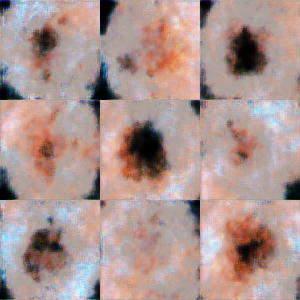
\includegraphics[width=\textwidth]{4.png}
        \caption{200 epochs.}
        \label{fig:1}
    \end{subfigure}
~
    \begin{subfigure}[t]{0.15\textwidth}
             \centering

        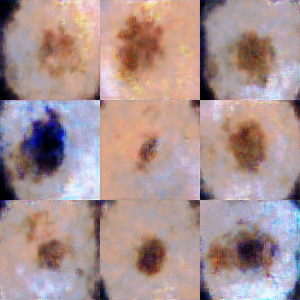
\includegraphics[width=\textwidth]{5.png}
        \caption{400 epochs.}
        \label{fig:2}
    \end{subfigure}
~
    \begin{subfigure}[t]{0.15\textwidth}
             \centering

        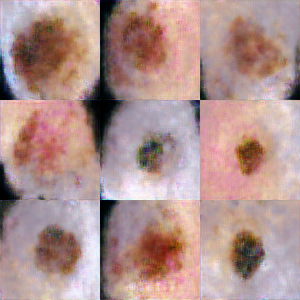
\includegraphics[width=\textwidth]{6.png}
        \caption{600 epochs.}
        \label{fig:3}
    \end{subfigure} 
  ~     
   
    \begin{subfigure}[b]{0.15\textwidth}
        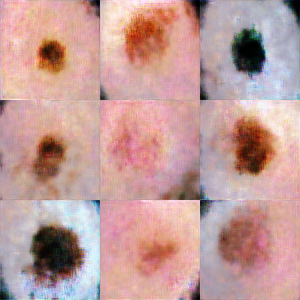
\includegraphics[width=\textwidth]{7.png}
        \caption{800 epochs.}
        \label{fig:4}
    \end{subfigure}
  ~
    \begin{subfigure}[b]{0.15\textwidth}
        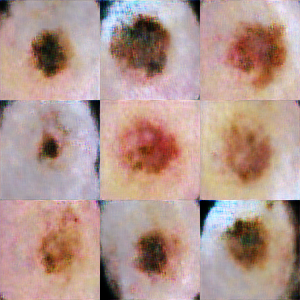
\includegraphics[width=\textwidth]{8.png}
        \caption{1000 epochs.}
        \label{fig:5}
    \end{subfigure}
    ~
    \begin{subfigure}[b]{0.15\textwidth}
        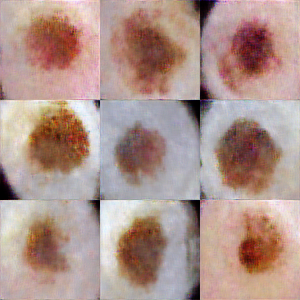
\includegraphics[width=\textwidth]{9.png}
        \caption{1200 epochs.}
        \label{fig:6}
    \end{subfigure}
   ~
     \begin{subfigure}[b]{0.15\textwidth}
        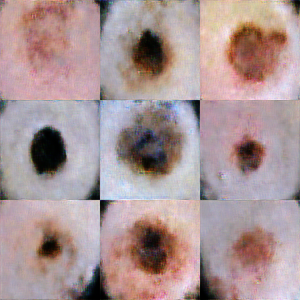
\includegraphics[width=\textwidth]{10.png}
        \caption{1400 epochs.}
        \label{fig:7}
    \end{subfigure}
   ~
    \begin{subfigure}[b]{0.15\textwidth}
        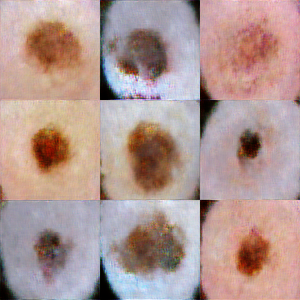
\includegraphics[width=\textwidth]{11.png}
        \caption{1600 epochs.}
        \label{fig:8}
    \end{subfigure}
  ~
    \begin{subfigure}[b]{0.15\textwidth}
        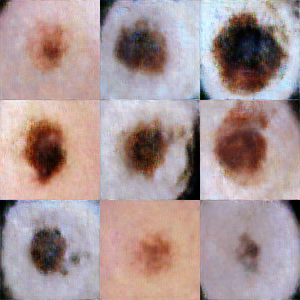
\includegraphics[width=\textwidth]{12.png}
        \caption{1800 epochs.}
        \label{fig:8}
    \end{subfigure} 
       
   ~
    \begin{subfigure}[b]{0.15\textwidth}
        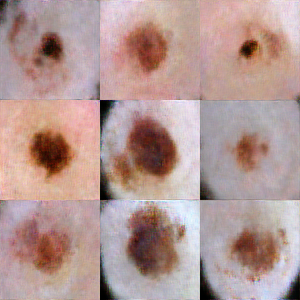
\includegraphics[width=\textwidth]{13.png}
        \caption{2000 epochs.}
        \label{fig:9}
    \end{subfigure}
  
    
    \caption{WGAN performance during 2000 epochs.}\label{fig:GANR}
\end{figure}


Then, in order to achieve better result the Wasserstein GAN(WGAN) algorithm is implemented on the data. The main difference between the GAN and WGAN can be regarded as, in the WGAN a new cost function using Wasserstein distance that has a smoother gradient everywhere is used, moreover, WGAN learns without paying attention to the generator act. 





\begin{figure}
\centering
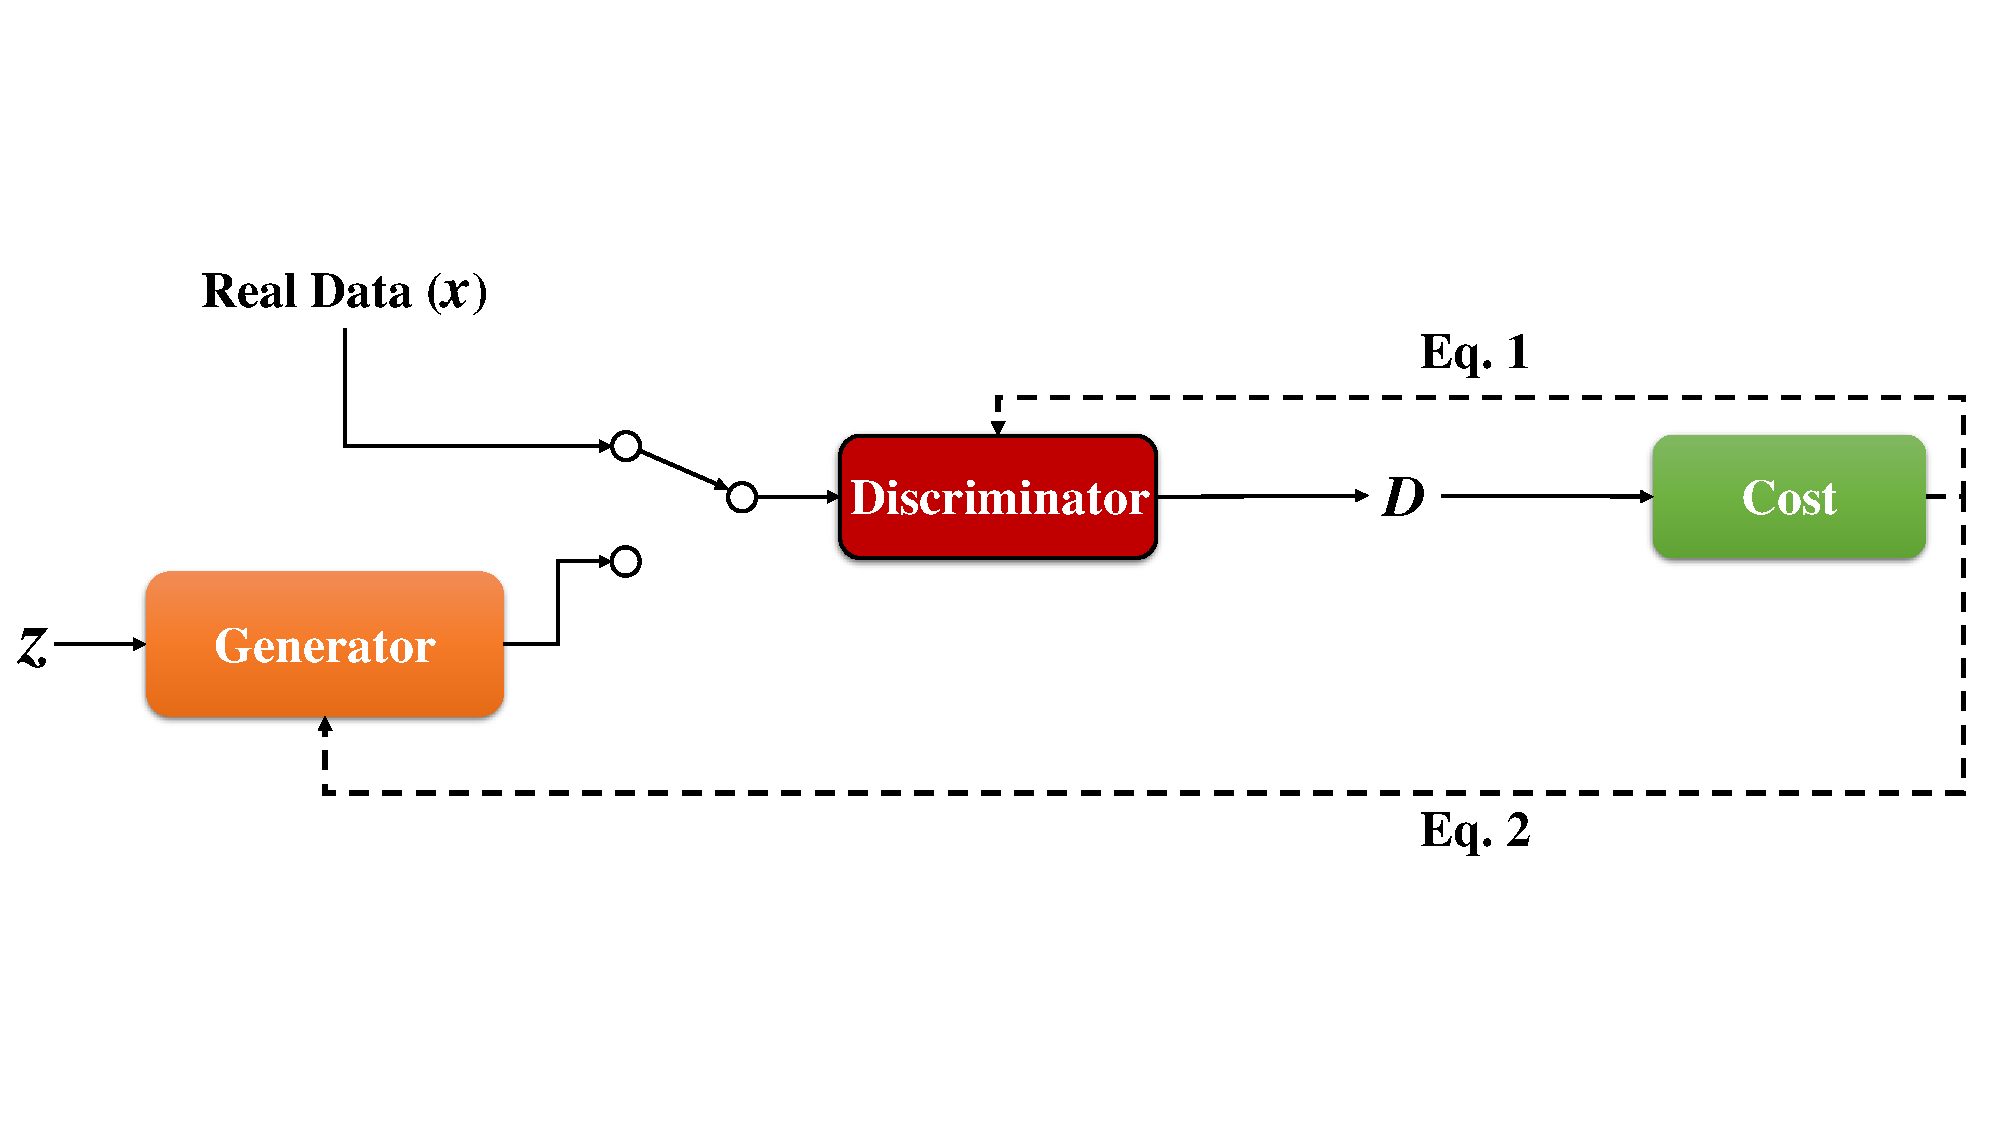
\includegraphics[width=1\columnwidth]{gan}
\caption{The GAN algorithm structure.}
\label{gann}
\centering
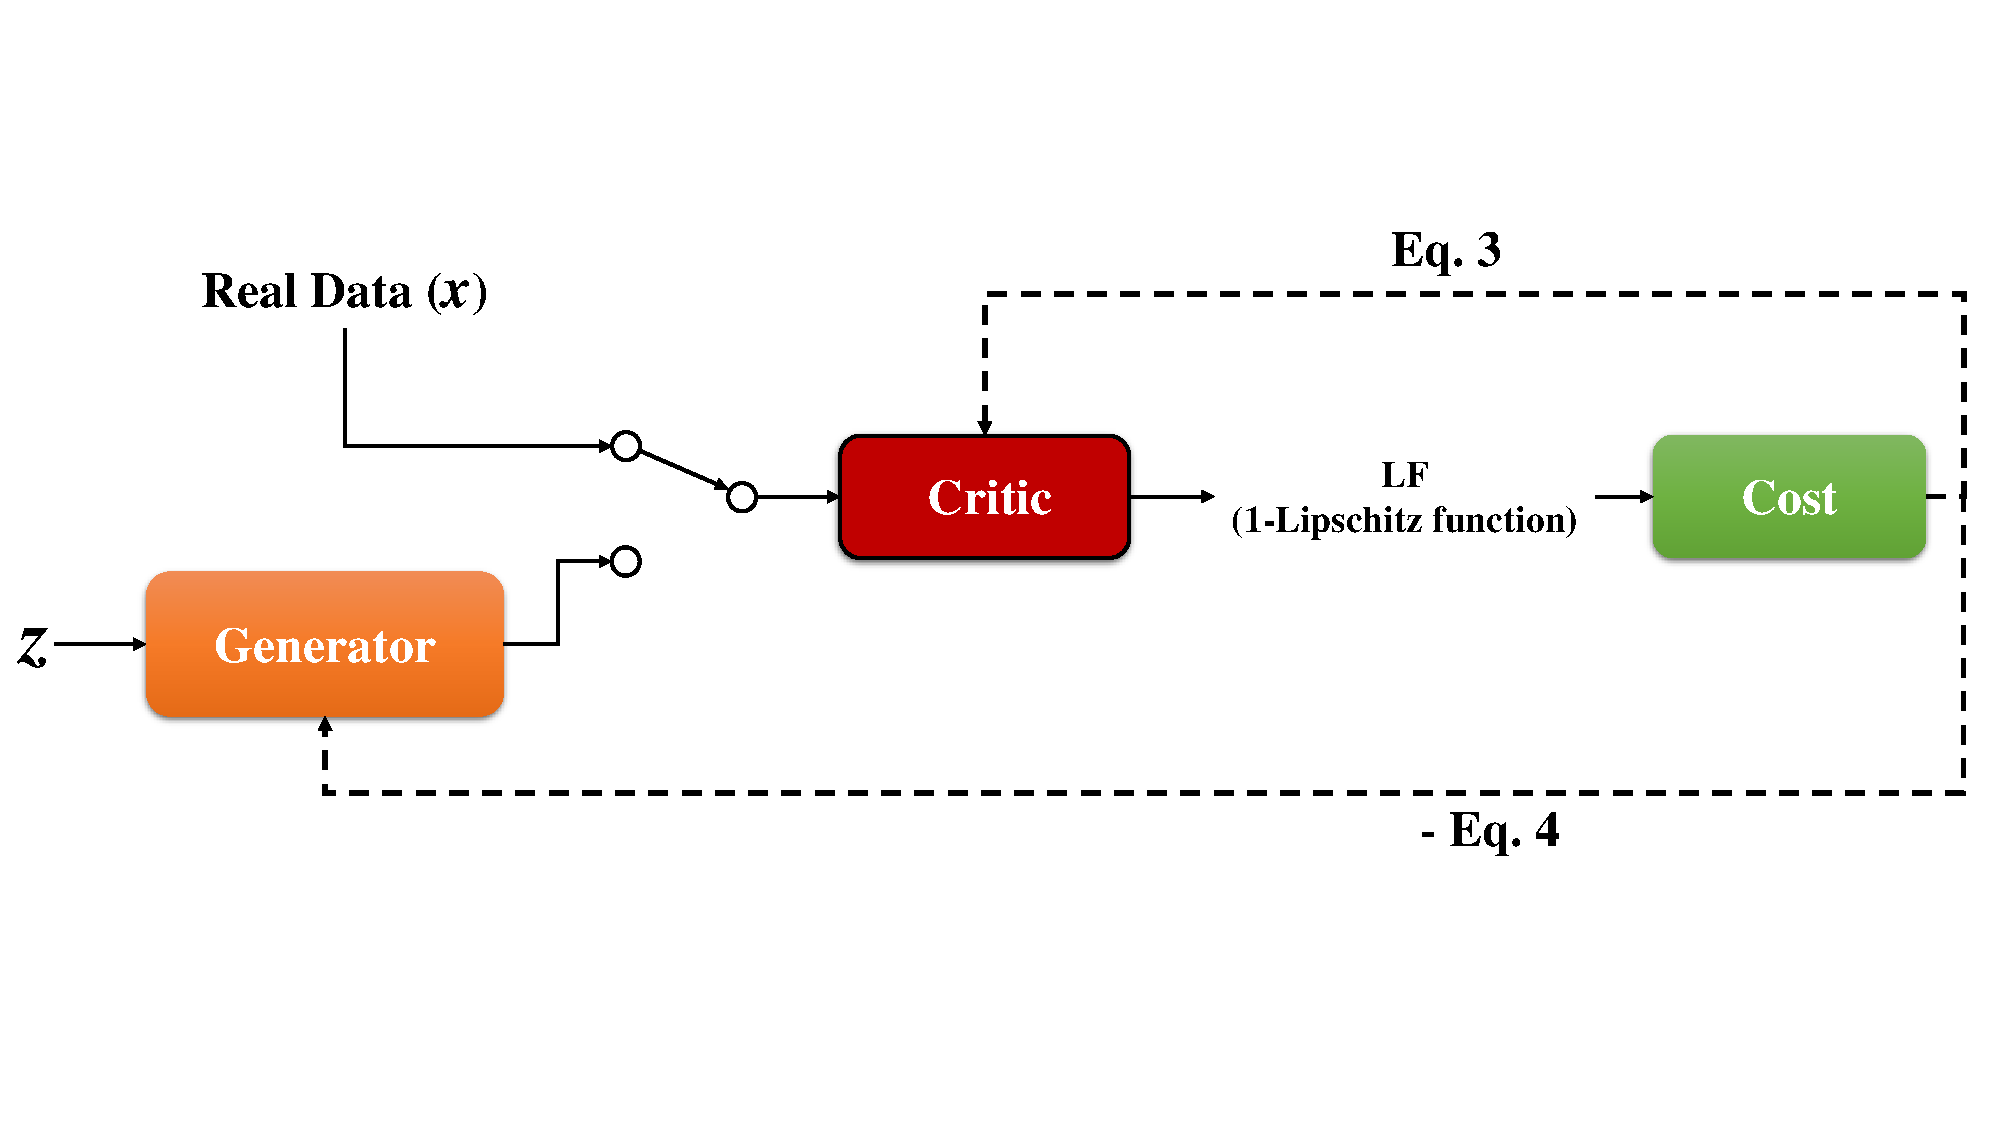
\includegraphics[width=1\columnwidth]{wgan}
\caption{The WGAN algorithm structure.}
\label{wgann}
\end{figure}

Figures~\ref{gann} and \ref{wgann} illustrate the stucture of GAN and WGAN algorithms.
the variables which are used in Eqs.~\ref{dgan},~\ref{ggan},~\ref{cwgan}	and \ref{gwgan} are defined as,$z$ is the noise which can consider as a normal or uniform distributions, $G$ , is the generator and it used to create an image based on $x=G(z)$. Moreover, $m$ is the number of noise and examples which are achieved from data generations, $D(x)$, is the function to calculate the probability that $x$ came from the data rather than gener<ator distribution.Furthermore,$\nabla$ is the stochastic gradient decent which is used to training the GAN based on $\theta_{d}$ and $\theta_{g}$ parameters.
Figure~\ref{itere} depicts the obtained images after $1000$ iterations.As it is obvious in the Fig.~\ref{itere}, after each $200$ iterations the quality of the images have been improved.

\begin{figure}
\centering
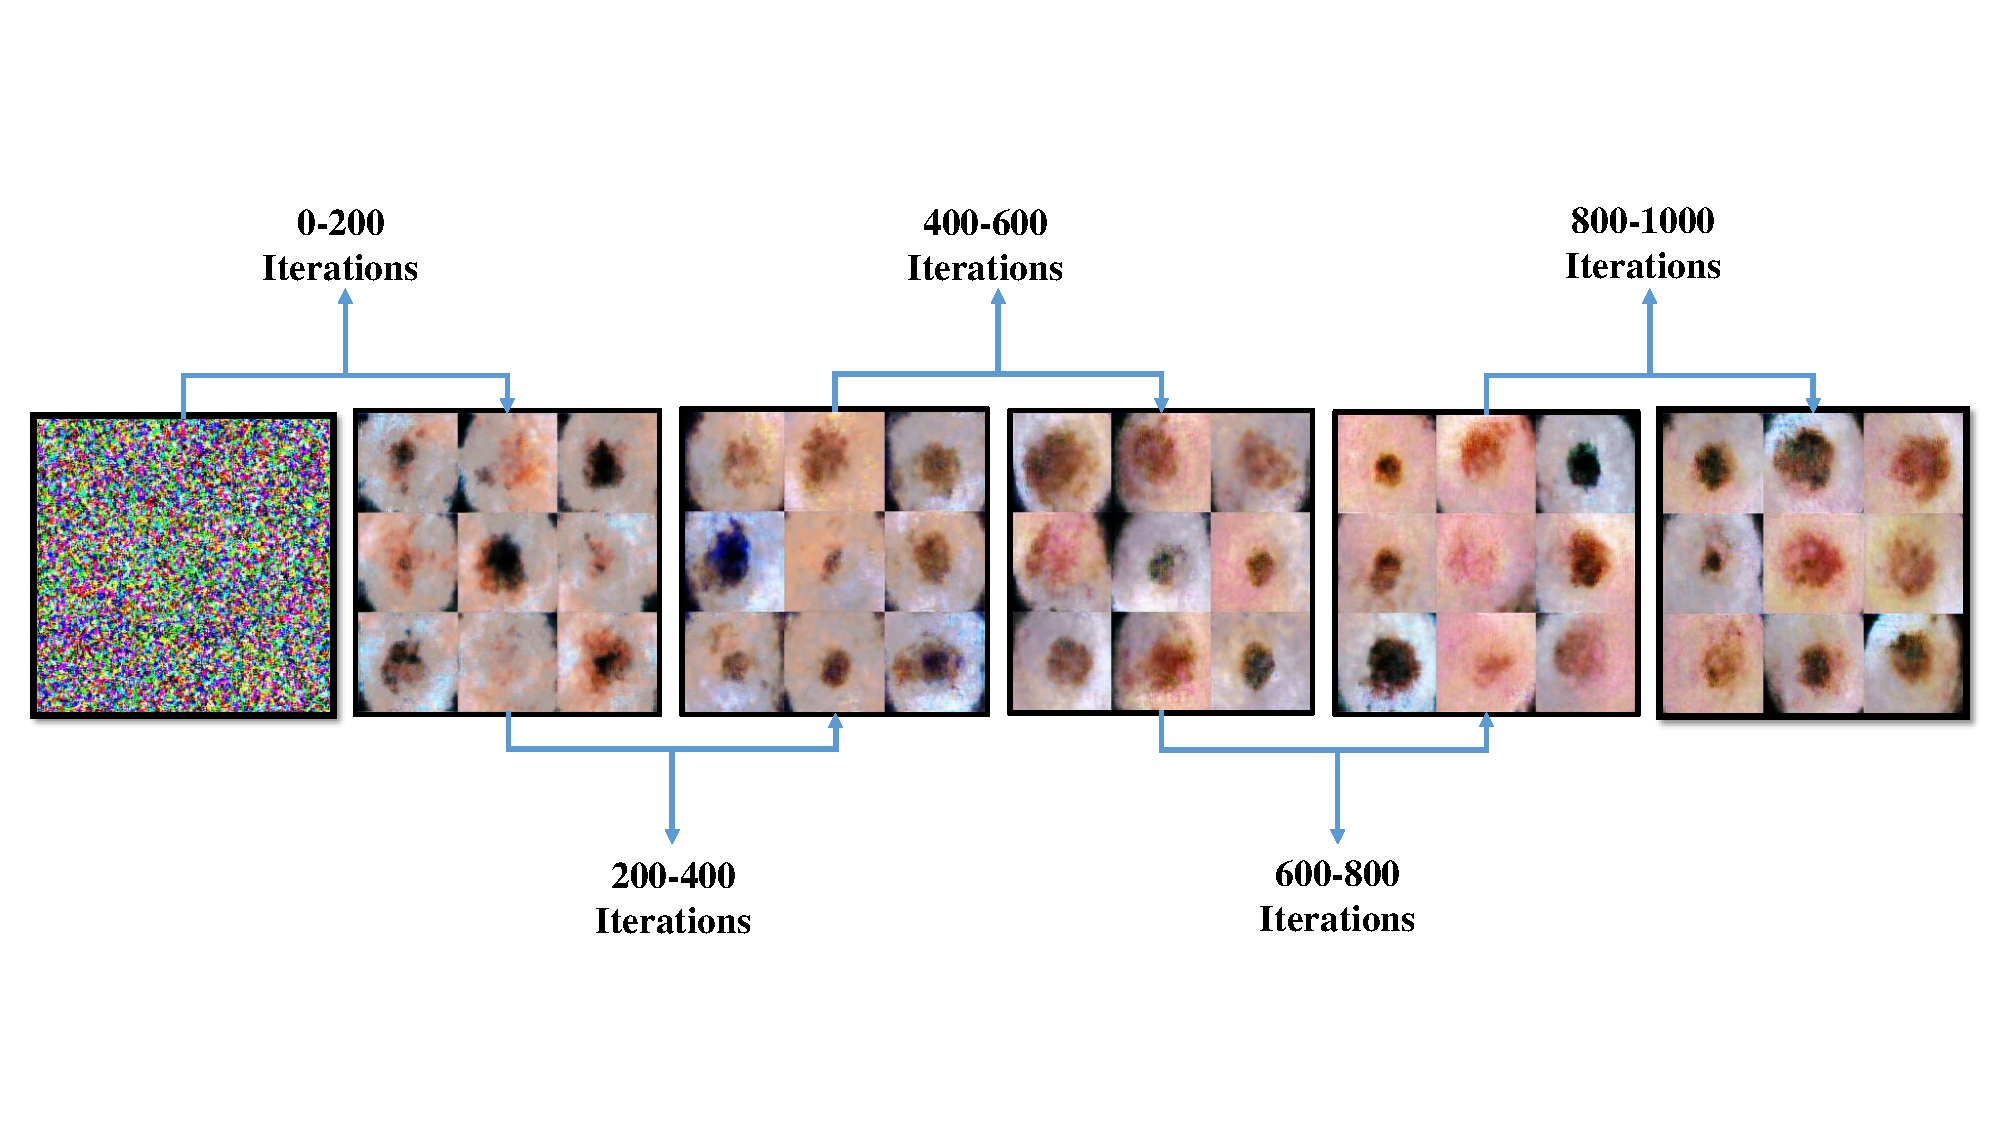
\includegraphics[width=1\columnwidth]{iteration.pdf}
\caption{The obtained result after $1000$ iterations of WGAN implementation.}
\label{itere}
\end{figure}


\subsection{Results}


\section{Model Training}


\subsection{Convlutional Neural Network}
In order to implement the convolutional neural network on the dataset, the
Keras libraries are used. The main steps to set the CNN algorithm on the
proposed dataset can be regarded as:
\begin{enumerate}
\item In order to initialize the neural network, the Sequential library is used.
\item In order to make the CNN for the images the Convolution2D is used.
\item The pooling layers are added by using of MaxPooling2D (Reduce the size
of the feature map).
\item The Flatten function is set to convert the pooled feature map to a single
column that is passed to the fully connected layer (All the pooled feature
maps are taken and put into a single vector).
\item The Dense function is used to added fully connected layer to the neural network (Using the input vector for the neural network).
Listing 1 illustrates the process of setting the parameters and functions to design the CNN algorithm.
\end{enumerate}


\subsection{Results}

\section{Discussion}

\section{Conclusion}
In this report the process of implementing the WGAN algorithm is represented and the main reasons that prove the superiority of the WGAN compare to the GAN algorithm are represented. Moreover, some of the results which are obtained based on the implementation of WGAN are illustrated. Furthermore, the process of designing and implementing the convlotional neural network on the generated databse is described. Based on the results which are obtained from the CNN algorithm implementation, after 300 epochs the accuracy of the training model is 63 percentages which can considered as a so good results by considering the number of the under study database and the number of epochs. Now, the process of collecting data, generalizing new data, making model and
testing the model is finished and the next step is writing a paper by combining the technical reports which are prepared in three versions.

\begin{thebibliography}{00}
%\bibitem{1} Ferlay J SI, Ervik M, Dikshit R, Eser S, Mathers C, Rebelo M,
%Parkin DM, Forman D, Bray, F, ``Cancer Incidence and
%Mortality Worldwide: IARC CancerBase,'' No 11. http://globocan.
%iarc.fr, 2013.
%
%\bibitem{2} Shirazi AZ, Chabok SJ, Mohammadi Z.,``A novel and reliable computational intelligence system for breast cancer detection,'' Medical \& biological engineering \& computing. 2018 May 1;56(5):721-32.

\bibitem{3} Khuriwal N, Mishra N. , ``Breast cancer diagnosis using adaptive voting ensemble machine learning algorithm,'' In 2018 IEEMA Engineer Infinite Conference (eTechNxT) 2018 Mar 13 (pp. 1-5). IEEE.

\bibitem{4} Deng C, Perkowski M., ``A Novel Weighted Hierarchical Adaptive Voting Ensemble Machine Learning Method for Breast Cancer Detection,'' In 2015 IEEE International Symposium on Multiple-Valued Logic (ISMVL) 2015 May 1 (pp. 115-120). IEEE.

\bibitem{5} Qasem A, Abdullah SN, Sahran S, Wook TS, Hussain RI, Abdullah N, Ismail F.,``Breast cancer mass localization based on machine learning,'' In Signal Processing \& its Applications (CSPA), 2014 IEEE 10th International Colloquium on 2014 Mar 7 (pp. 31-36). IEEE.

\bibitem{6} Gayathri BM, Sumathi CP. , ``Comparative study of relevance vector machine with various machine learning techniques used for detecting breast cancer,'' In Computational Intelligence and Computing Research (ICCIC), 2016 IEEE International Conference on 2016 Dec 15 (pp. 1-5). IEEE.
  
\bibitem{7} Forsyth AW, Barzilay R, Hughes KS, Lui D, Lorenz KA, Enzinger A, Tulsky JA, Lindvall C., ``Machine learning methods to extract documentation of breast cancer symptoms from electronic health records,''Journal of pain and symptom management. 2018 Jun 1;55(6):1492-9.

\bibitem{8} Nayak S, Gope D., ``Comparison of supervised learning algorithms for RF-based breast cancer detection,'' In Computing and Electromagnetics International Workshop (CEM), 2017 2017 Jun 21 (pp. 13-14). IEEE.

\bibitem{9} Kim S, Jung S, Park Y, Lee J, Park J., ``Effective liver cancer diagnosis method based on machine learning algorithm,'' In Biomedical Engineering and Informatics (BMEI), 2014 7th International Conference on 2014 Oct 14 (pp. 714-718). IEEE.

\bibitem{10} Turgut S, Dağtekin M, Ensari T., ``Microarray breast cancer data classification using machine learning methods,'' In 2018 Electric Electronics, Computer Science, Biomedical Engineerings' Meeting (EBBT) 2018 Apr 18 (pp. 1-3). IEEE.

%\bibitem{11} Chaurasia V, Pal S, Tiwari BB., ``Prediction of benign and malignant breast cancer using data mining techniques,'' Journal of Algorithms \& Computational Technology. 2018 Jun;12(2):119-26.
%\bibitem{12} Wang H, Zheng B, Yoon SW, Ko HS., ``A support vector machine-based ensemble algorithm for breast cancer diagnosis,'' European Journal of Operational Research. 2018 Jun 1;267(2):687-99.
% 
\bibitem{13} Zheng B, Yoon SW, Lam SS., ``Breast cancer diagnosis based on feature extraction using a hybrid of K-means and support vector machine algorithms,'' Expert Systems with Applications. 2014 Mar 1;41(4):1476-82.



\bibitem{14} de Vos, B.D., Wolterink, J.M., de Jong, P.A., Viergever, M.A. and Išgum, I., ``2D image classification for 3D anatomy localization: employing deep convolutional neural networks,'' In Medical Imaging 2016: Image Processing (Vol. 9784, p. 97841Y). International Society for Optics and Photonics.


\bibitem{15} Dou, Q., Yu, L., Chen, H., Jin, Y., Yang, X., Qin, J. and Heng, P.A., ``3D deeply supervised network for automated segmentation of volumetric medical images,''  2017, Medical image analysis, 41, pp.40-54.

\bibitem{16} Pan, Y., Huang, W., Lin, Z., Zhu, W., Zhou, J., Wong, J. and Ding, Z., ``Brain tumor grading based on neural networks and convolutional neural networks,'' In 2015 37th Annual International Conference of the IEEE Engineering in Medicine and Biology Society (EMBC) (pp. 699-702). IEEE.



\bibitem{17} Abdel-Zaher, A.M. and Eldeib, A.M., ``Brain tumor grading based on neural networks and convolutional neural networks,'' 2016, Breast cancer classification using deep belief networks. Expert Systems with Applications, 46, pp.139-144.


\bibitem{18} Cheng, J.Z., Ni, D., Chou, Y.H., Qin, J., Tiu, C.M., Chang, Y.C., Huang, C.S., Shen, D. and Chen, C.M., ``Computer-aided diagnosis with deep learning architecture: applications to breast lesions in US images and pulmonary nodules in CT scans,'' 2016, Scientific reports, 6, p.24454.


\end{thebibliography}



\end{document}
